\documentclass[a4paper,14pt]{extarticle} 
\usepackage[a4paper,top=1.5cm, bottom=1.5cm, left=2cm, right=1cm]{geometry}
%\usepackage[T2A]{fontenc}
%\usepackage[english, russian]{babel}
\usepackage{graphicx}
\DeclareGraphicsExtensions{.pdf,.png,.jpg}

\usepackage{fontspec}
\setmainfont{Times New Roman}
\setsansfont{FreeSans}
\setmonofont{FreeMono}
\renewcommand{\baselinestretch}{1.5}
\usepackage{polyglossia}
\setdefaultlanguage{russian}
\setotherlanguages{english,russian}
\usepackage{setspace}
\usepackage[many]{tcolorbox}
\usepackage{listings}
\usepackage{xcolor}
\usepackage{pdfpages}

\definecolor{codegreen}{rgb}{0,0.6,0}
\definecolor{codegray}{rgb}{0.5,0.5,0.5}
\definecolor{codepurple}{rgb}{0.58,0,0.82}
\definecolor{backcolour}{rgb}{0.95,0.95,0.92}

\lstdefinestyle{mystyle}{
    backgroundcolor=\color{backcolour},   
    keywordstyle=\color{magenta},
    numberstyle=\tiny\color{codegray},
    stringstyle=\color{codepurple},
    basicstyle=\ttfamily\footnotesize,
    breakatwhitespace=false,         
    breaklines=true,                 
    captionpos=b,                    
    keepspaces=true,                 
    numbers=left,                    
    numbersep=5pt,                  
    showspaces=false,                
    showstringspaces=false,
    showtabs=false,                  
    tabsize=2
}

\lstset{style=mystyle}

\begin{document}
    \begin{center}
        \thispagestyle{empty}
        \begin{singlespace}
        ФЕДЕРАЛЬНОЕ АГЕНТСТВО СВЯЗИ

        ФЕДЕРАЛЬНОЕ ГОСУДАРСТВЕННОЕ БЮДЖЕТНОЕ ОБРАЗОВАТЕЛЬНОЕ

        УЧРЕЖДЕНИЕ ВЫСШЕГО ОБРАЗОВАНИЯ

        «САНКТ-ПЕТЕРБУРГСКИЙ ГОСУДАРСТВЕННЫЙ УНИВЕРСИТЕТ ТЕЛЕКОММУНИКАЦИЙ ИМ. ПРОФ. М.А. БОНЧ-БРУЕВИЧА»

        (СПбГУТ)
        \end{singlespace}
        \vspace{-1ex}
        \rule{\textwidth}{0.4pt}
        \vspace{-5ex}

        Факультет \underline{Инфокоммуникационных сетей и систем}

        Кафедра \underline{Защищенных систем связи}
        \vspace{10ex}

        \textbf{Лабораторная работа №1}\\
        


    \end{center}
    \vspace{4ex}
    \begin{flushright}
    \parbox{10 cm}{
    \begin{flushleft}
        Выполнили студенты группы ИКТЗ-83:

        \underline{Громов А.А., Миколаени М.С., Мазеин Д.С.} \hfill \rule[-0.85ex]{0.1\textwidth}{0.6pt}

        \footnotesize \textit{ (Ф.И.О., № группы) \hfill (подпись)} \normalsize

        Проверил:

        \underline{Казанцев А.А.} \hfill \rule[-0.85ex]{0.1\textwidth}{0.6pt}

        (\footnotesize \textit{уч. степень, уч. звание, Ф.И.О.) \hfill (подпись)} \normalsize

    \end{flushleft}
    }
    \end{flushright}
    \begin{center}
        \vfill
        Санкт-Петербург

        2021

    \end{center}
    \newpage

    \textbf{Цель лабораторной работы:}

    Перенести в autocad, добавить систему охраны:
    \vspace{-6ex}
    \begin{singlespace}
        \begin{itemize}
            \item расположить охранные датчики,
            \item расположить камеры, 
            \item расположить СКУД.
        \end{itemize} 
    \end{singlespace}

    \textbf{Схема помещения:}
    \begin{center}
        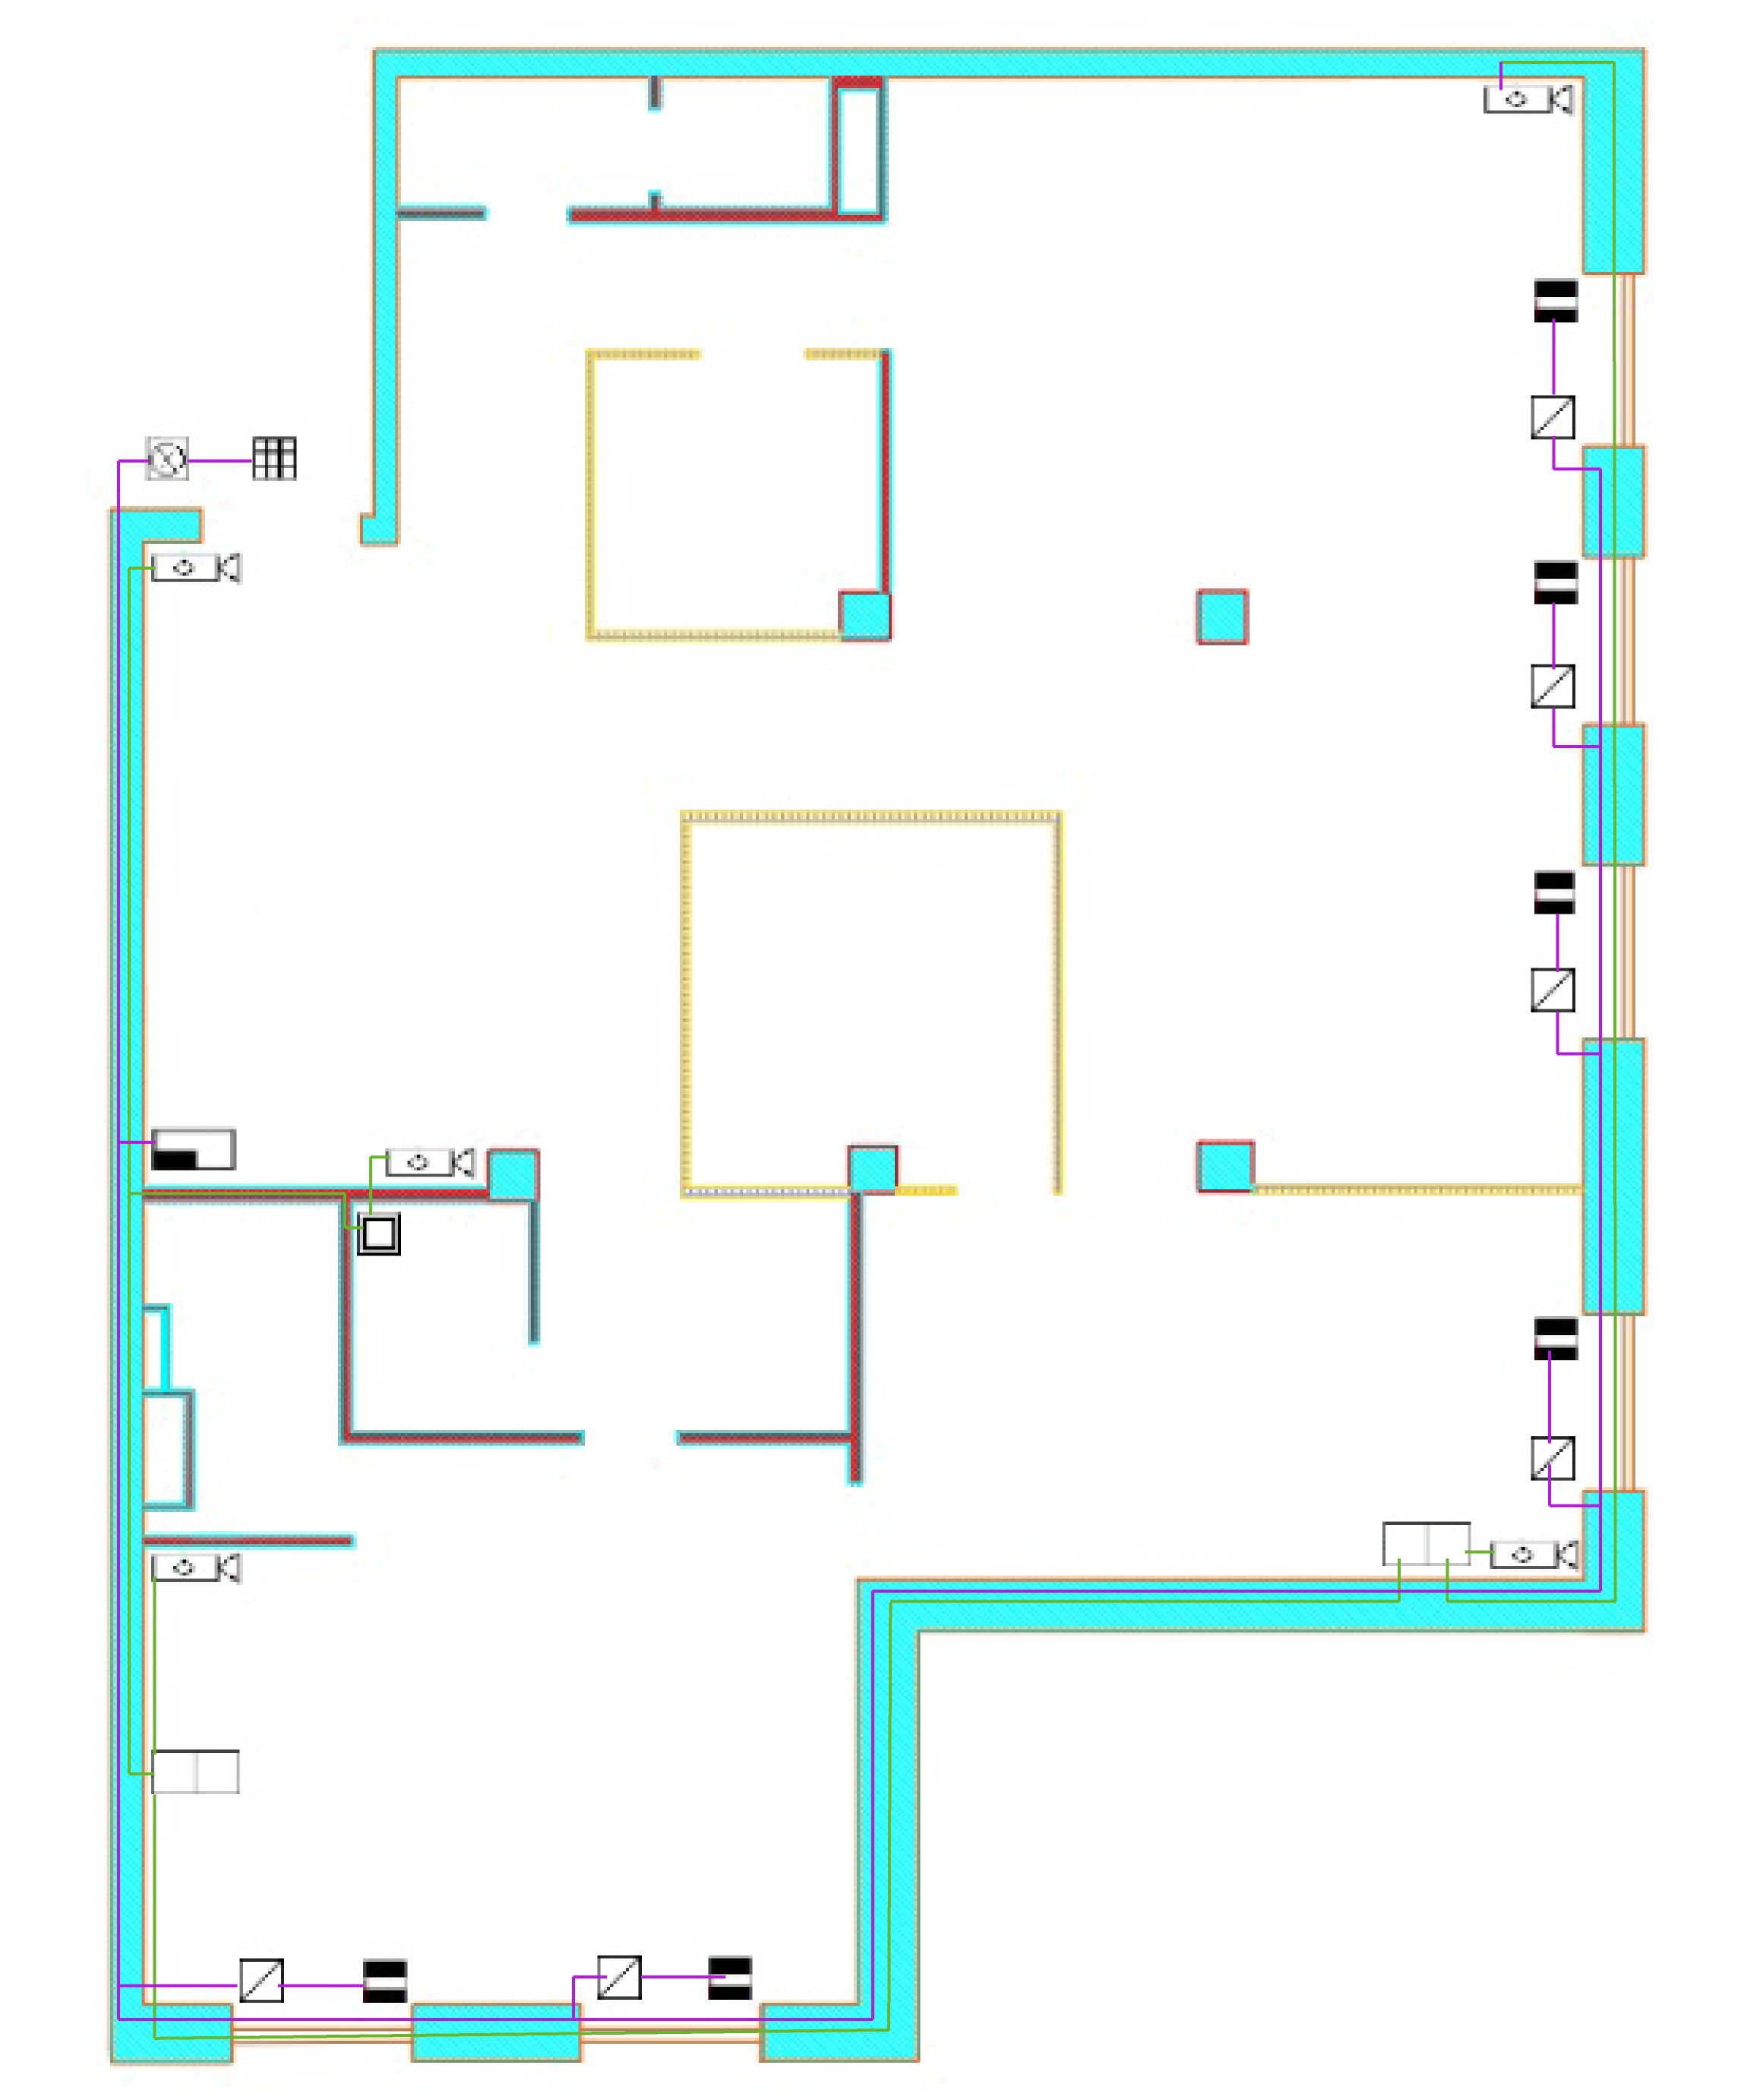
\includegraphics[scale=0.6, angle=90]{pics/scheme.png}
    \end{center}

    \newpage
    \textbf{\large{Охранная сигнализация}}

    \begin{center}
        \textbf{Схема}
    \end{center}
    \vspace{-6ex}
    \begin{center}
        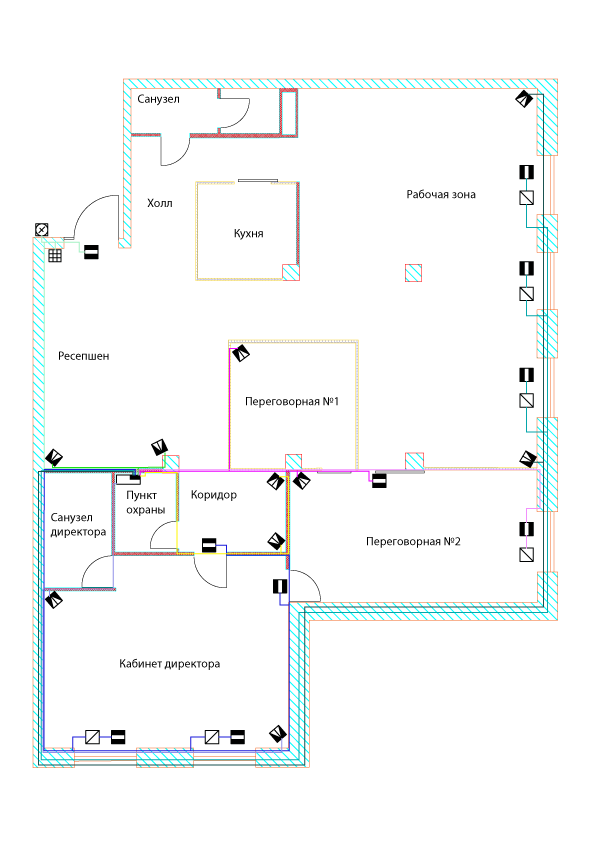
\includegraphics[scale=0.65, angle=90]{pics/Sensors.png}
    \end{center}
    \textbf{Условные обозначения}
    \begin{center}
        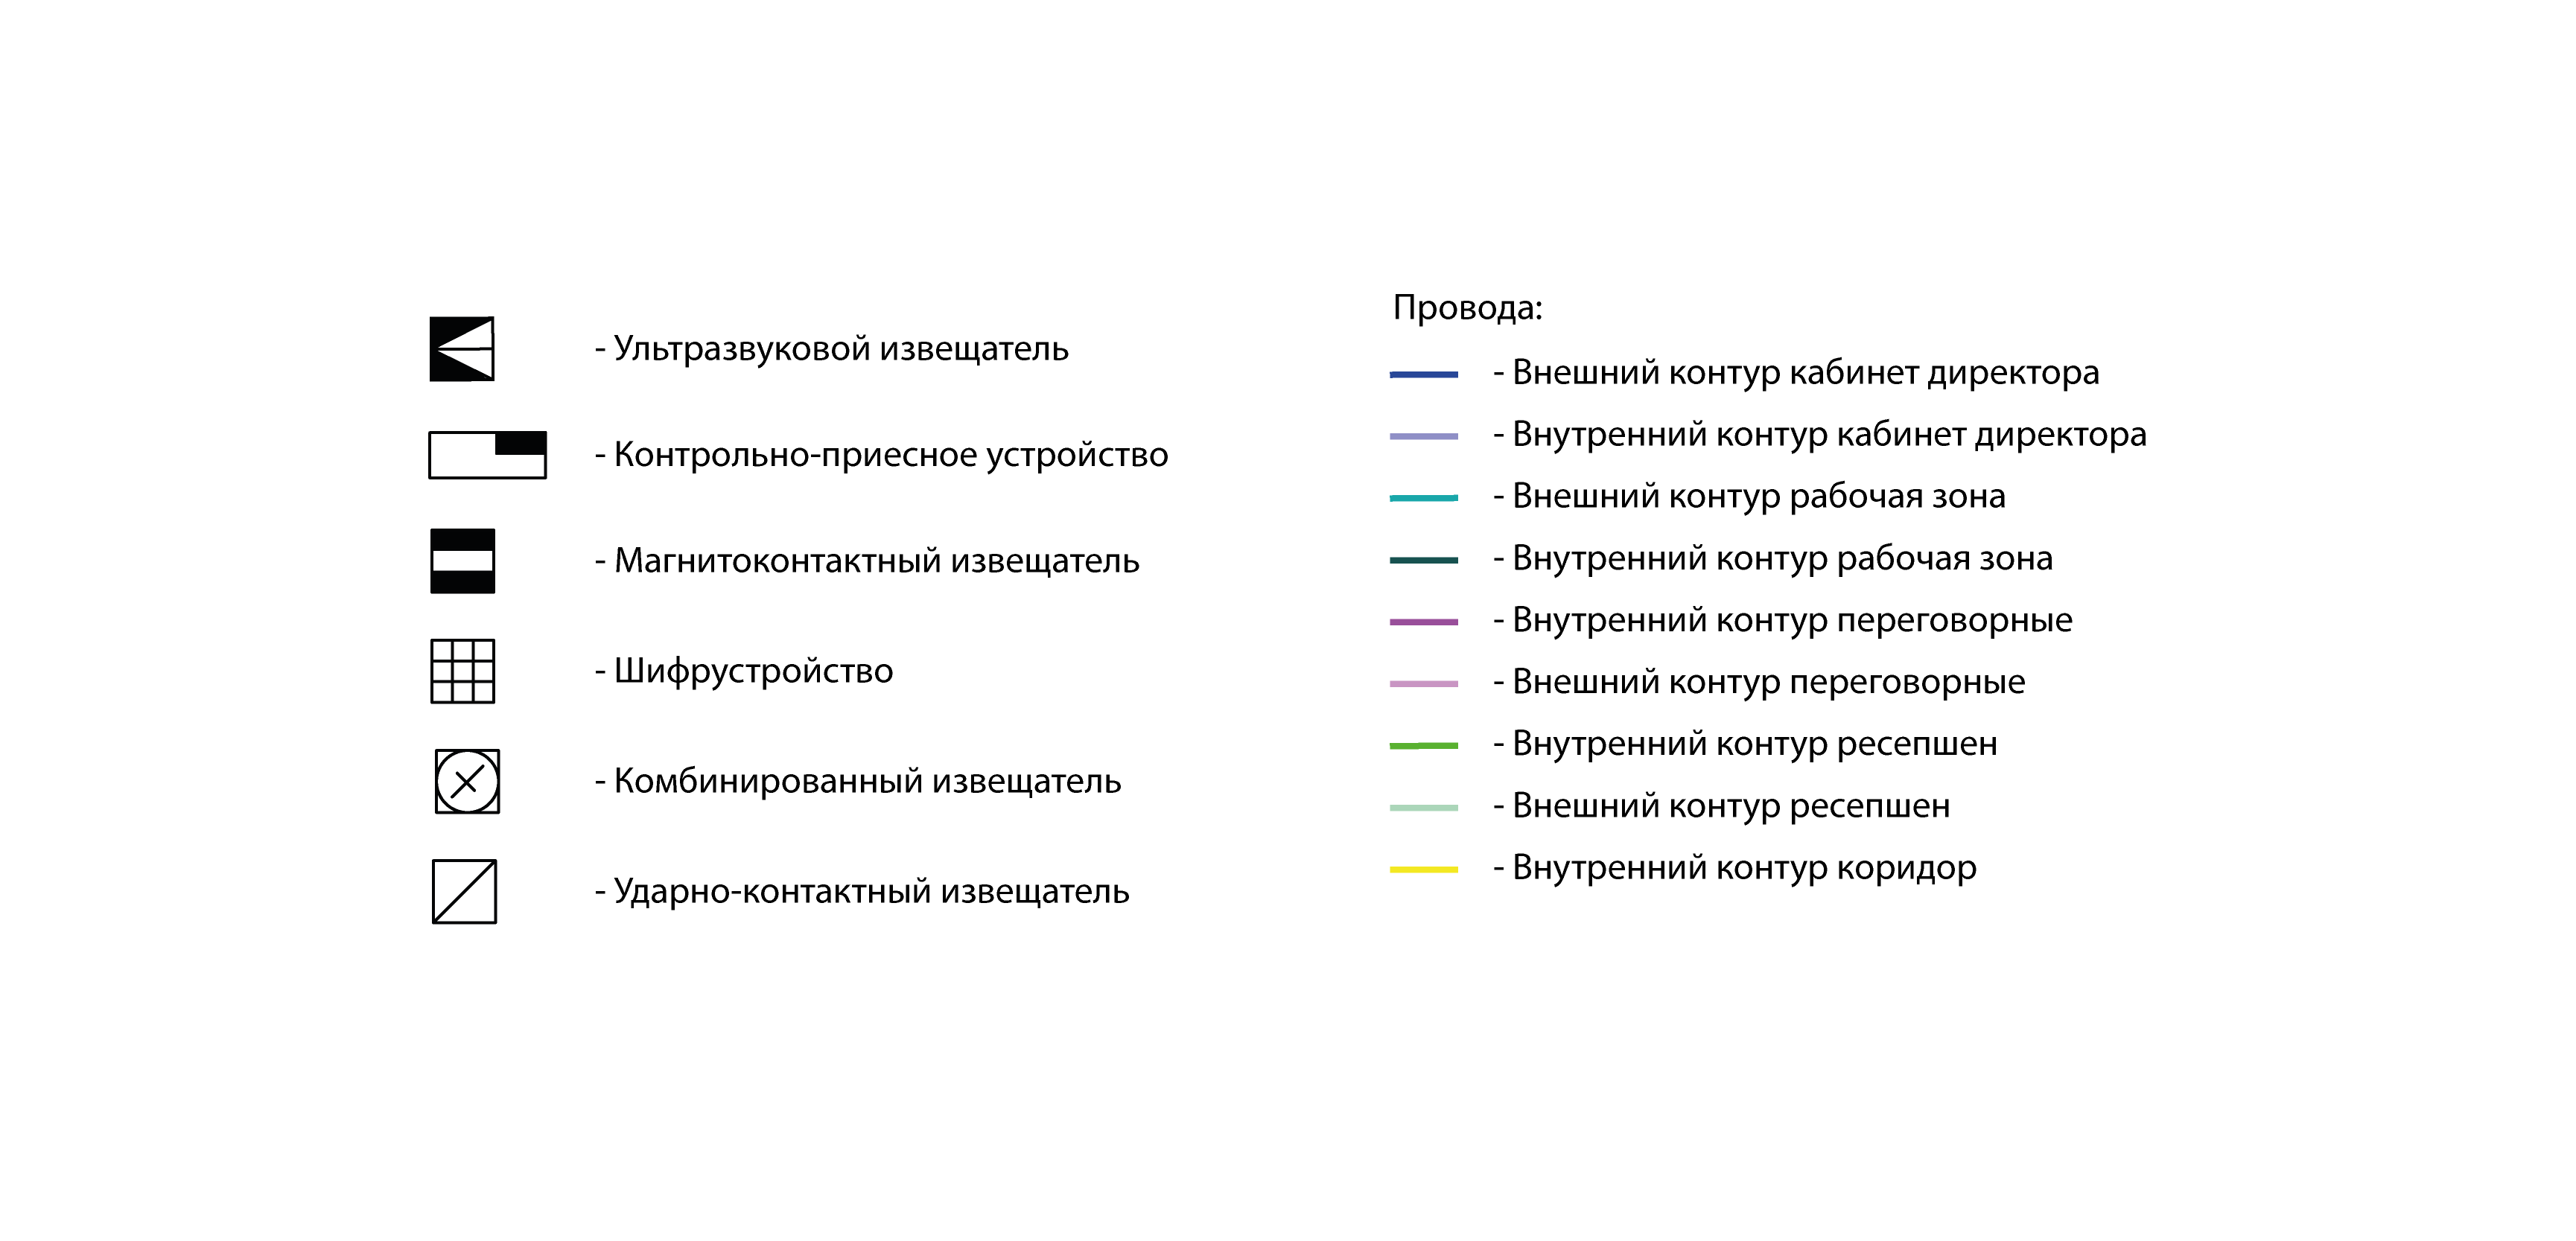
\includegraphics[scale=0.65]{pics/Sensors(mark).png}
    \end{center}
    \textbf{Пояснительная записка}
    \begin{spacing}{1.25}
        Офисное помещение разделено на 5 зоны:
        \vspace{-1ex}
        \begin{spacing}{0.5}
            \begin{itemize}
                \item рабочая зона;
                \item ресепшн;
                \item переговорные; 
                \item коридор;
                \item кабинет директора;
            \end{itemize}
        \end{spacing}
        Четыре зоны(Рабочая зона, ресепшн. переговорная, кабинет директора) разделены на 2 клонтура:
        \begin{spacing}{0.5}
            \begin{itemize}
                \item внешний, состоящий из ударно-контактных и магнитоконтактных извещателей
                \item внутренний, состоящий из ультразвуковых извещателей 
            \end{itemize}
        \end{spacing}
        На респешене дополнительно во внешний контур добавлены шифрустройство и комбинироанный оповещатель
        Коридор включает в себя один контур - внутренний, состоящий из ультразвуковых извещателей
    \end{spacing}
    
    \newpage
    \textbf{\large{Система видеонаблюдения}}

    \begin{center}
        \textbf{Схема}
    \end{center}
    \vspace{-6ex}
    \begin{center}
        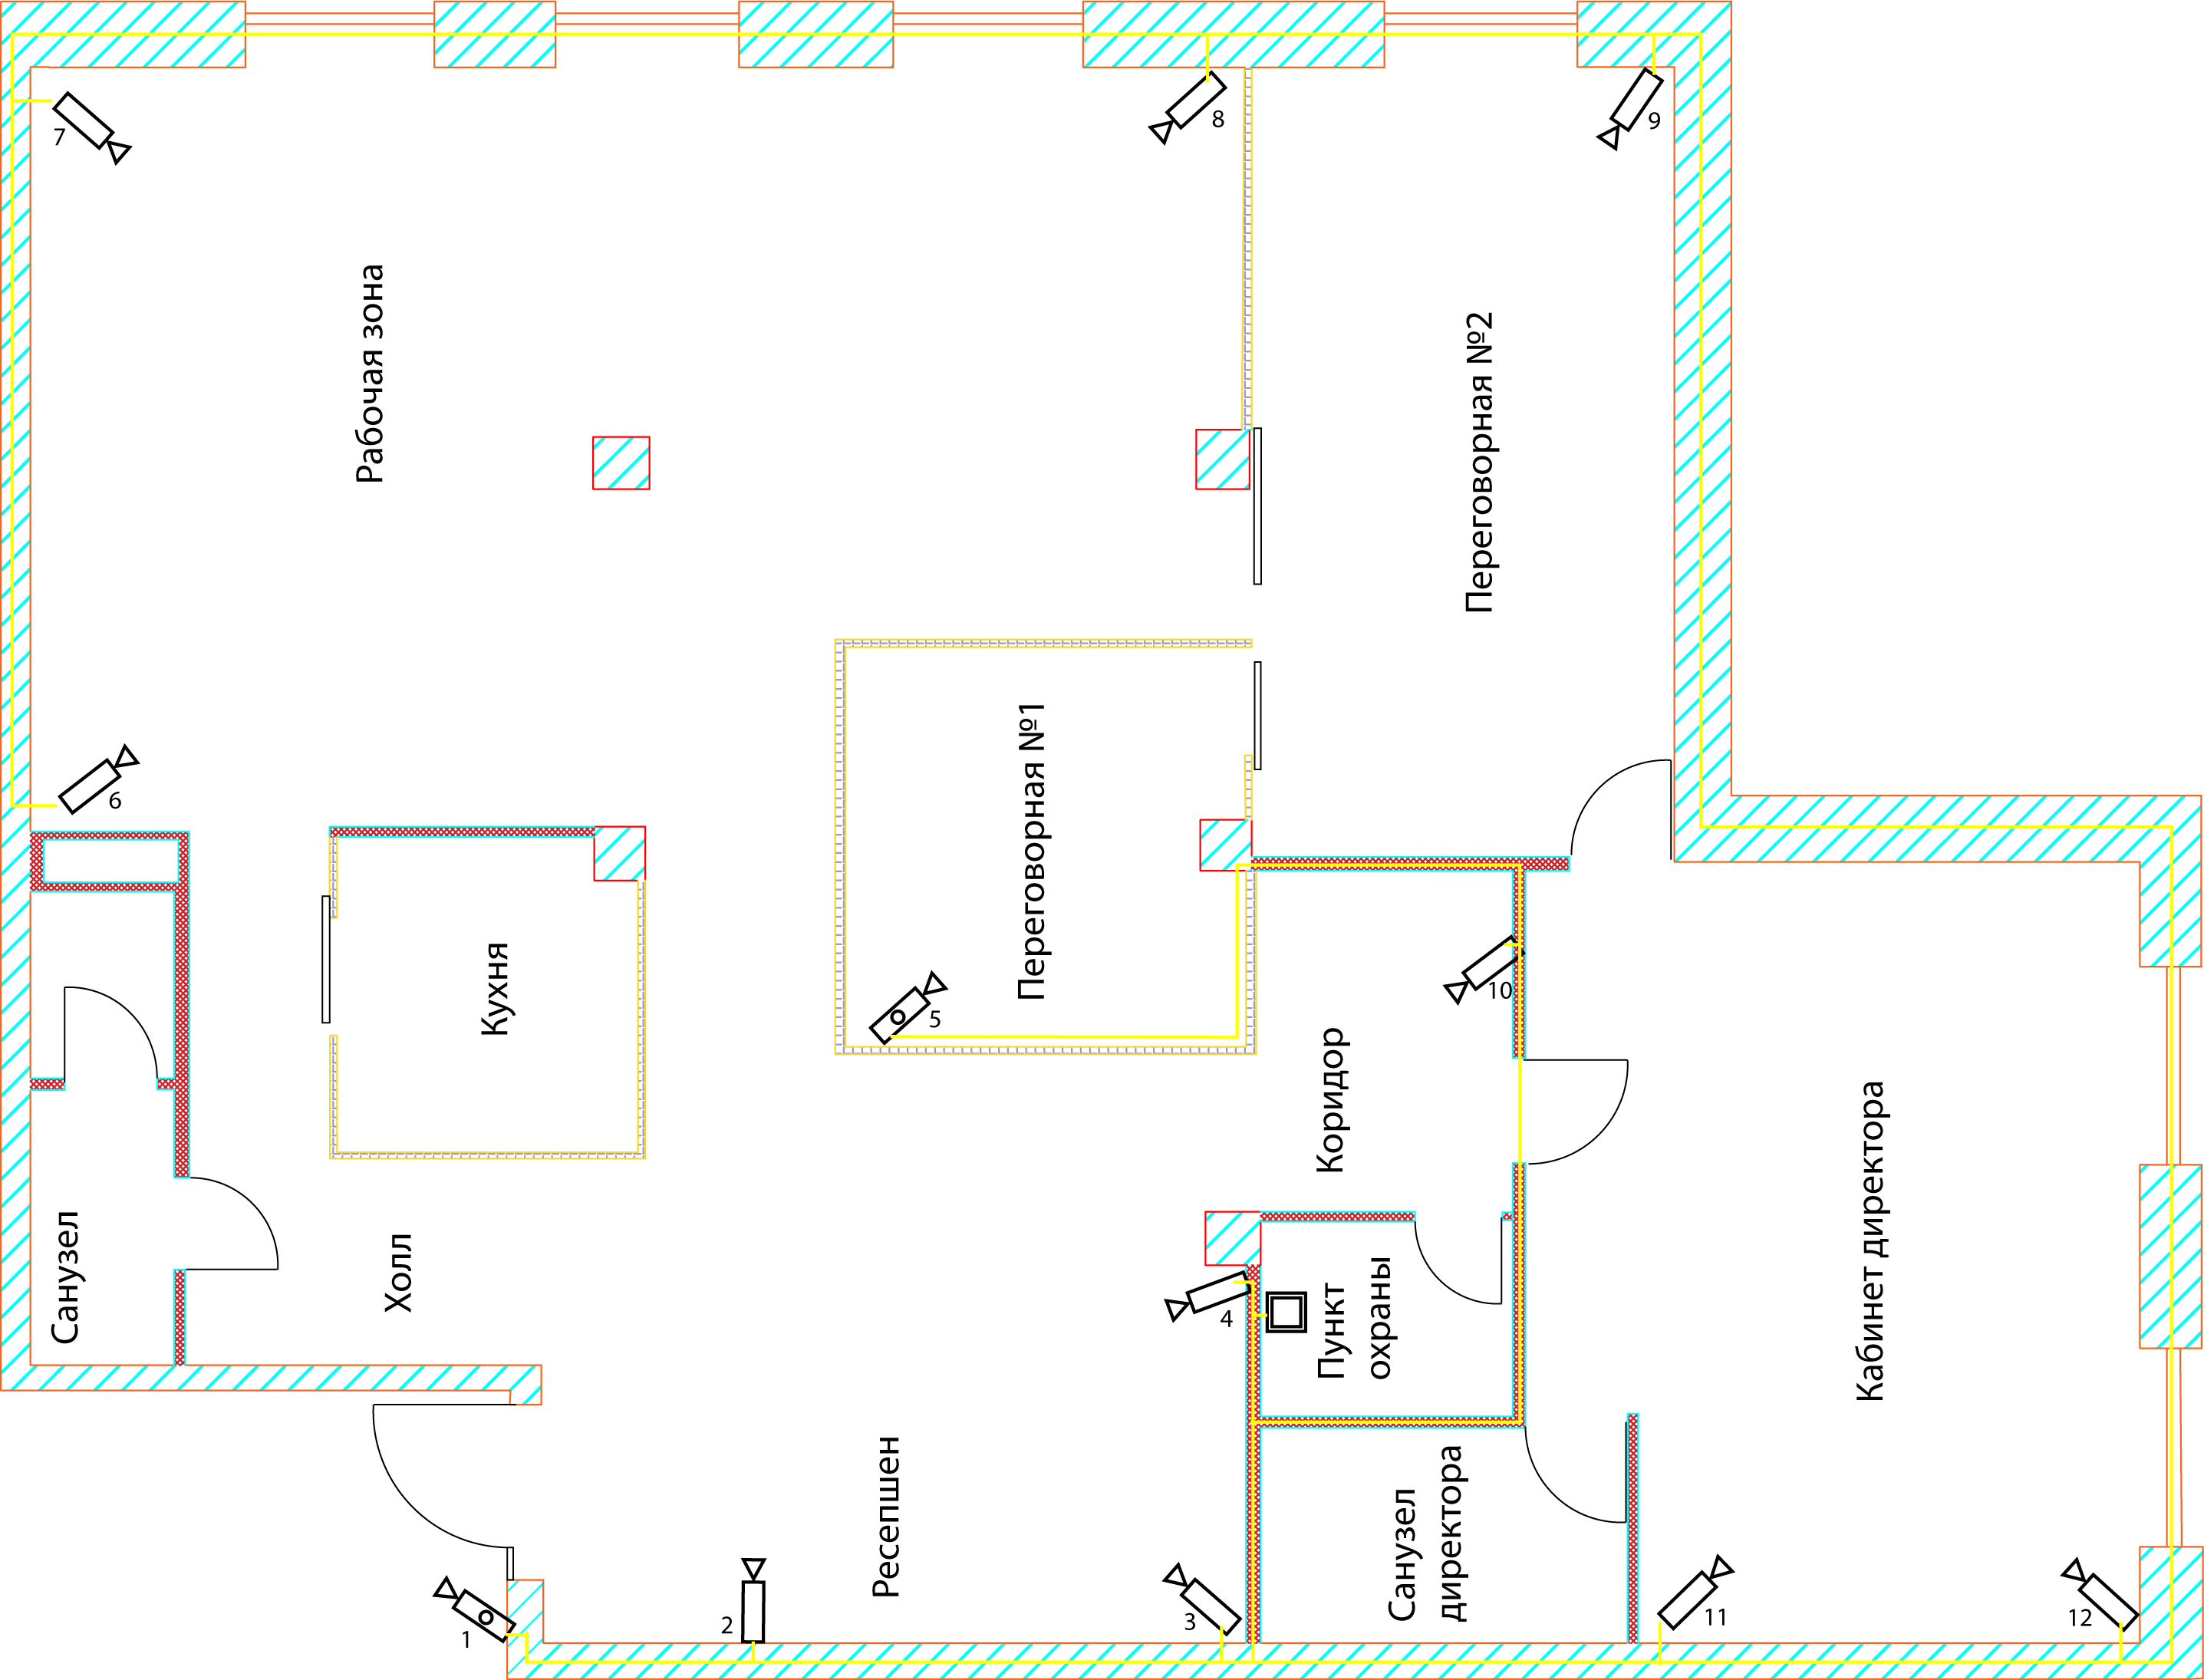
\includegraphics[scale=0.65]{pics/Cams.png}
    \end{center}
    \textbf{Условные обозначения}
    \begin{center}
        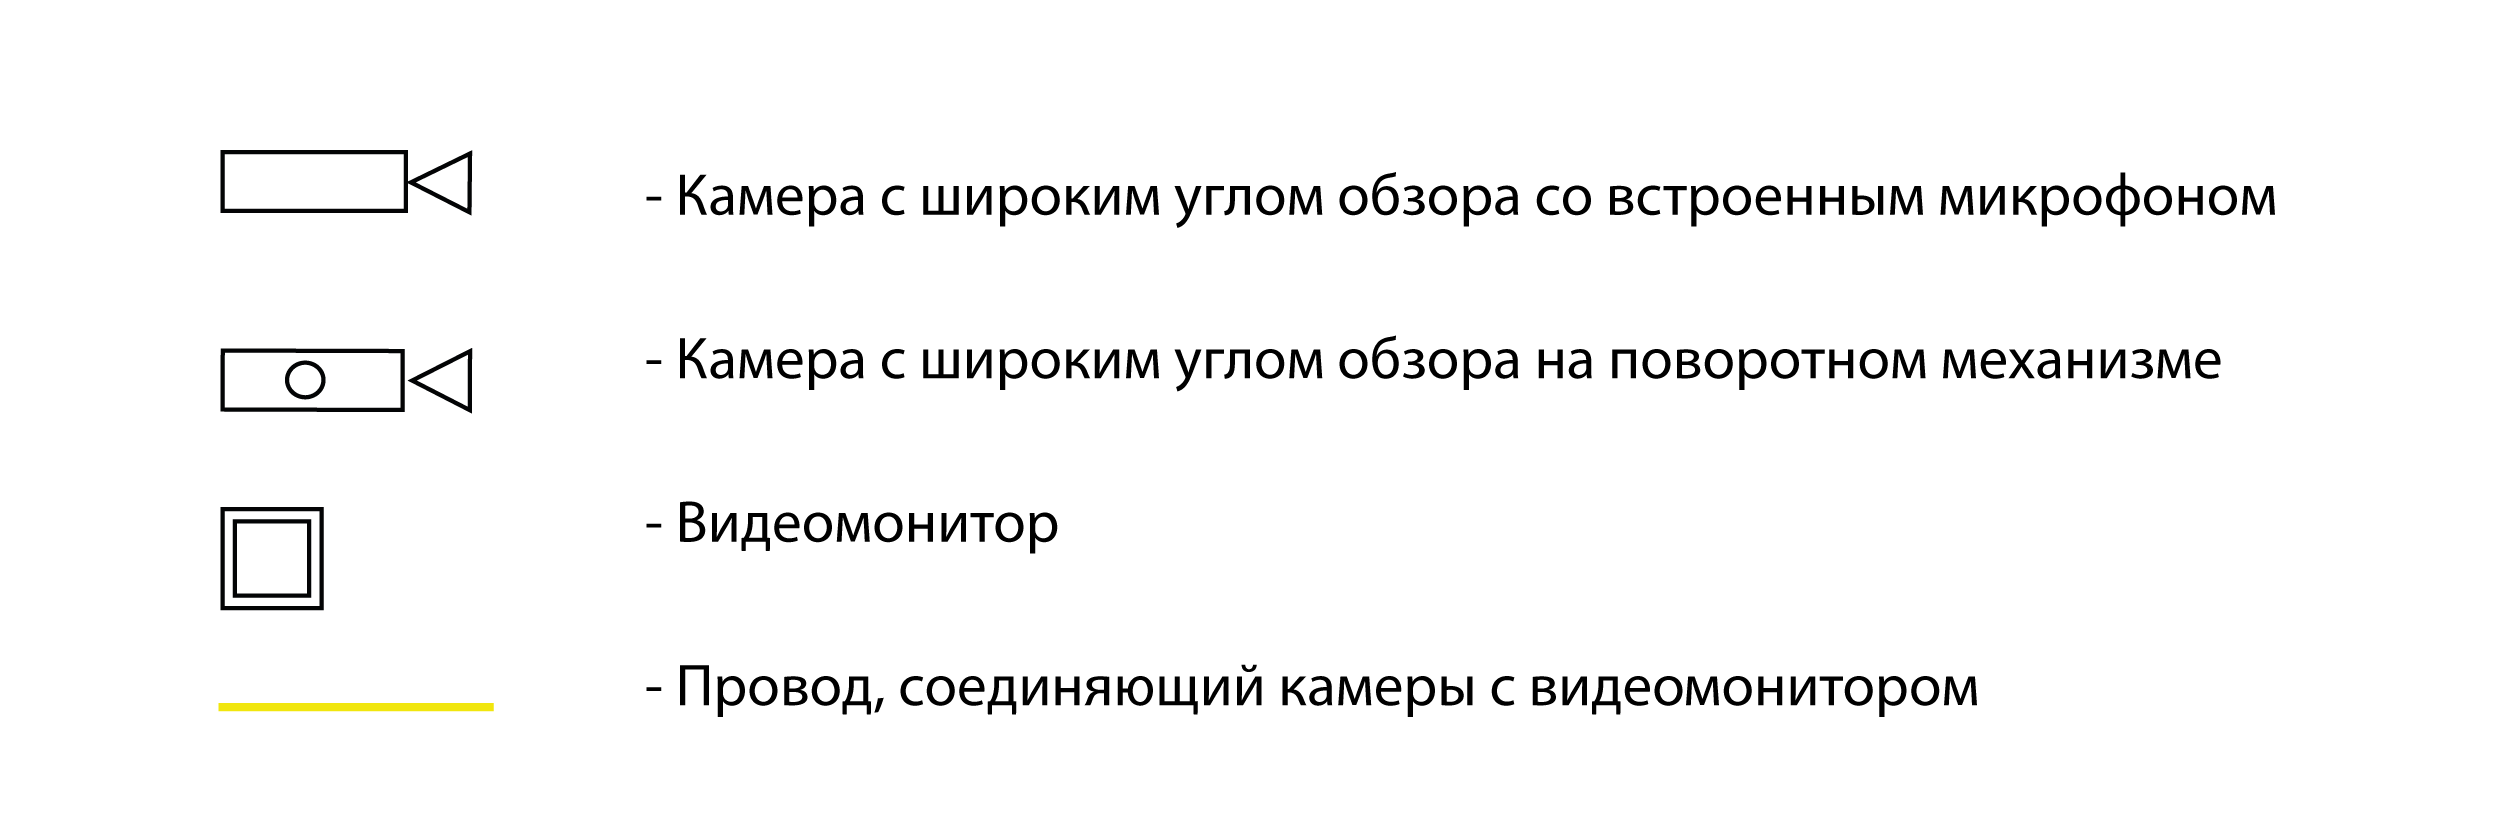
\includegraphics[scale=0.65]{pics/Cams(mark).png}
    \end{center}
    \textbf{Пояснительная записка}
    \begin{spacing}{1.25}
        Поворотная камера на входе позволяет отслеживать подходящих к входной двери людей.

        Камеры, установленные на респешене просматривают коридор между кухней и переговорной №1, холл, а также контролируют входную дверь.

        Камеры, расположенные в рабочей зоне отслеживают перемещения сотрудников на рабочих местах. 

        Камеры, установленные в переговорных позволяют наблюдать за людьми, которые находятся в данных комнатах.

        Камера в коридоре контролирует проход к пункту охраны и кабинету директора.

        Камеры, в кабинете директора позволяют отслеживать действия лиц, находящихся в кабинете, а также происходящее за окнами офиса. 
    \end{spacing}

    \newpage
    \textbf{\large{Система контроля и управления доступом}}

    \begin{center}
        \textbf{Схема}
    \end{center}
    \vspace{-6ex}
    \begin{center}
        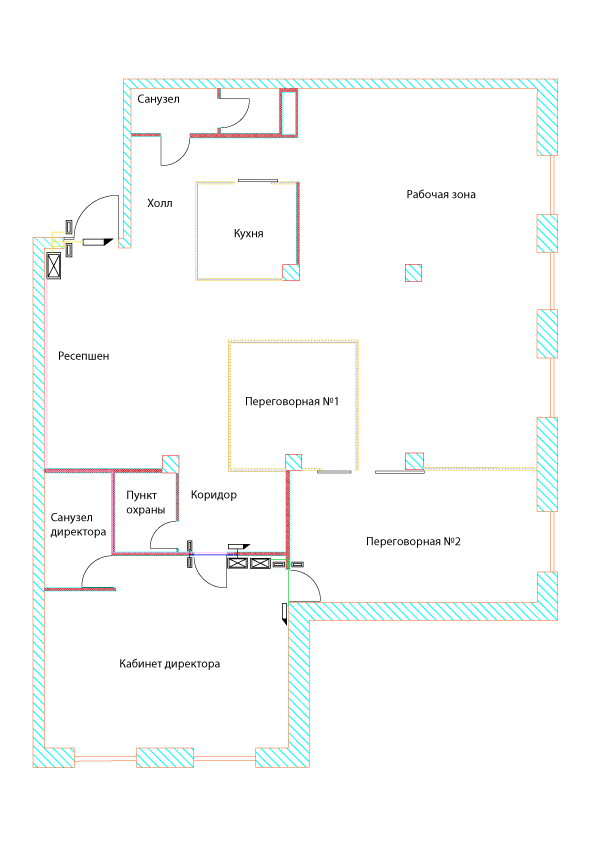
\includegraphics[scale=0.65, angle=90]{pics/SCUD.png}
    \end{center}
    \textbf{Условные обозначения}
    \begin{center}
        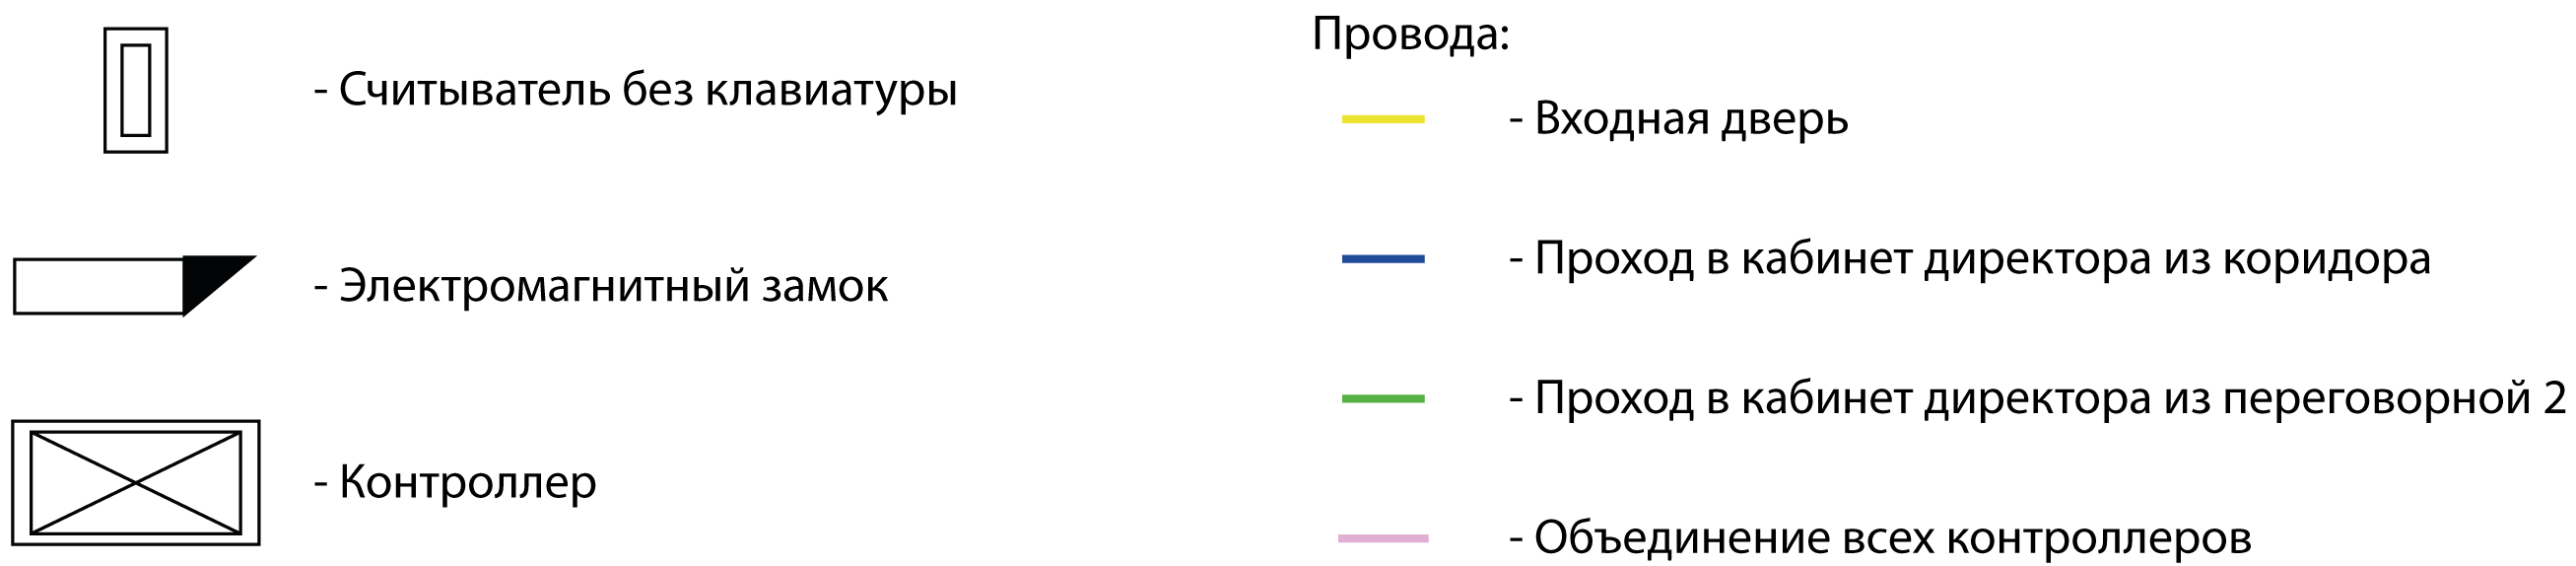
\includegraphics[scale=0.65]{pics/SCUD(mark).png}
    \end{center}
    \textbf{Пояснительная записка}
    \begin{spacing}{1.25}
        Офис распологает 3 системами контроля и управления доступом:
        \vspace{-1ex}
        \begin{spacing}{0.5}
            \begin{itemize}
                \item на входной двери в офис;
                \item на двери в кабинет директора из коридора;
                \item на двери в кабинет директора из переговорной №2.
            \end{itemize}
        \end{spacing}
        Каждая система состоит из контроллера, электромагнитного замка и считывателя без клавиатуры.\\ 
        Все системы объединены в единую сеть.
    \end{spacing}



 
    


    
    


\end{document}